\documentclass{article} % For LaTeX2e
\usepackage{nips15submit_e,times}
\usepackage{hyperref}
\usepackage{url}
%\documentstyle[nips14submit_09,times,art10]{article} % For LaTeX 2.09
%Example for automatically rescaling equations. 
% This is very tricky.
%\begin{equation}
%\label{eq:pimax}
%\resizebox{.55\textwidth}{!}{$
%\begin{split}
%P(\jtable_{2}|\set{E},\ttable) \propto &
%P(\keys = [jack,101],\it{Gr} = A, \it{Sat} = 1|\it{Int} = \class, \it{Rank} = 1, \it{Rat} = 3, \it{Diff}=1)\\
%\times & P(\keys = [jack,102],\it{Gr} = B, \it{Sat} = 2|\it{Int} = \class, \it{Rank} = 1, \it{Rat} = 2, \it{Diff}=2).
%\end{split}$
%}
%\end{equation}

%\usepackage{times}
%\usepackage[normaltitle,normalbib,normalmargins,normalindent]{savetrees}
\usepackage{amsmath}
\usepackage{amsfonts}
\usepackage{amssymb}
\usepackage{graphicx}
\usepackage{url}
%\usepackage{subfigure}
\usepackage{epstopdf}
\setcounter{MaxMatrixCols}{30}
%\usepackage{algorithm}
%\usepackage{algorithmic}
\usepackage{subfigure}
%\usepackage{subcaption}
\usepackage{fancyhdr}
\graphicspath{{../}{figures/}}
\usepackage{todonotes}

\DeclareMathOperator*{\argmax}{argmax}
\DeclareMathOperator*{\argmin}{argmin}
%\DeclareMathOperator{\pattern}{\pi}
\DeclareMathOperator{\Poly}{\mathbf{\mathrm{P}}}
\DeclareMathOperator{\RP}{\mathbf{\mathrm{RP}}}
%\DeclareMathOperator{\FP}{\mathbf{\mathrm{FP}}}
\DeclareMathOperator{\NP}{\mathbf{\mathrm{NP}}}
%\DeclareMathOperator{\E}{\mathbb{E}}
\renewcommand{\d}{\mathbf{d}}

\newcommand{\ZZ}{\mathbf{Z}}

\newcommand{\indep}{\ensuremath{\perp{}\!\!\!\!\!\!\!\perp{}}}
\newcommand{\dep}{\ensuremath{{\perp{}\!\!\!\!\!\!\!\not  \perp{}}}}
%\renewcommand{\L}{\mathcal{L}}
% variables denoting sets of nodes
\newcommand{\V}{V} 
\newcommand{\partC}{\mathcal{C}}
\newcommand{\pattern}{\pi}
% variables denoting nodes
\newcommand{\B}{B}
\renewcommand{\P}{P}
\newcommand{\R}{R}
\newcommand{\X}{X}
\newcommand{\Y}{Y}
\newcommand{\Z}{Z}
\newcommand{\F}{F}
\newcommand{\U}{U}
\newcommand{\W}{W}
\renewcommand{\S}{S}
\newcommand{\C}{C}
\newtheorem{mydef}{Proposition}
%variables for values
%\newcommand{\u}{u}
\renewcommand{\a}{a}
\renewcommand{\b}{b}
\newcommand{\z}{z}
\renewcommand{\v}{v}
\newcommand{\x}{x}
\newcommand{\y}{y}
\newcommand{\p}{p}
\newcommand{\s}{s}
\newcommand{\w}{w} % weights


%statistics
\newcommand{\divergence}{\it{D}}
\newcommand{\score}{\it{score}}
\newcommand{\confidence}{\it{conf}}
\newcommand{\support}{\it{support}}
\newcommand{\loglikelihood}{\it{LOG}}
\newcommand{\lof}{\it{LOF}}
\newcommand{\llmetric}{-L}
\newcommand{\lr}{\it{LR}}
\newcommand{\kl}{\it{KL}}
\newcommand{\el}{\it{EL}}
\newcommand{\mi}{\it{MI}}
\renewcommand{\mid}{\it{ELD}}
\newcommand{\jid}{\it{JID}}
\newcommand{\roc}{\it{ROC}}
\newcommand{\outrank}{\it{OutRank}}
\newcommand{\knn}{\it{KNNOutlier}}
\newcommand{\auc}{\it{AUC}}
\newcommand{\eld}{\it{ELD}}
\newcommand{\fd}{\it{FD}}
\newcommand{\parameter}{\theta}
\newcommand{\parameters}{\bs{\parameter}}
\newcommand{\bic}{\mathit{BIC}}
%random variables and graphical models
% number of values in the domain of a random variable
% variables for BNs
\newcommand{\domvals}{k}
\newcommand{\nodevalue}{\v}
\newcommand{\parvalue}{\mathbf{\pi}} % a single assignment of values to a set of 
%parents
\newcommand{\parvals}{l} % number of values of parent state.
\renewcommand{\r}{r} % CP-table row
\newcommand{\nbhd}{{\mathsf {nbdh}}}
\newcommand{\child}{\mathit{child}}
\newcommand{\parent}{\mathit{pa}}
\newcommand{\parents}{\mathbf{pa}}
\newcommand{\Parents}{\mathbf{PA}}
\newcommand{\family}{F} % families, family formulas
\newcommand{\vpi}{\mathbf{pa}} % for vectors of variable assignments
\renewcommand{\l}{\ell} % class label
\newcommand{\states}{r} % number of states of a variable
%\newcommand{\value}{value}
\newcommand{\mb}{\set{mb}} % markov blanket of a variable, vector-valued
\newcommand{\ssize}{N} % number of rows in join table; size of sample
\newcommand{\mbstates}{m} % number of states in Markov blanket
\newcommand{\frequency}{fr}
\newcommand{\pseudo}{\ast}
\newcommand{\counts}{+}
\newcommand{\weighted}{\ast}
\newcommand{\halpern}{H}
\newcommand{\Thetaa}{\theta}
\newcommand{\instance}{I}

%logic notation
%\newcommand{\predicate}{\phi}
\newcommand{\functor}{f}
\newcommand{\outdomain}{V}
\newcommand{\indomain}{\Omega}
\newcommand{\variable}{X} % first-order variable
\newcommand{\population}{\mathcal{P}}
\newcommand{\entity}{x}
\newcommand{\formula}{\phi}
\newcommand{\formulas}{\mathcal{\phi}}
\newcommand{\literal}{l}
\newcommand{\conjunction}{\set{C}} % conjunction of literals
\newcommand{\fterm}{\f} % open function term
\newcommand{\fterms}{F} % set of function terms, also nodes in JBN
\newcommand{\term}{\sigma}
\newcommand{\Terms}{\bs{\sigma}}
\newcommand{\constant}{a}
\newcommand{\constants}{\bs{\constant}}
\newcommand{\gterm}{g} % ground term
\newcommand{\gterms}{\bs{\gterm}} %list of ground terms
\newcommand{\vterm}{x} % variable term
\newcommand{\vterms}{\bs{\vterm}} % list of variable terms
\newcommand{\assign}{A} % assignment of values to Bayes net
\newcommand{\resultset}{\mathbb{R}}
\newcommand{\grounds}{\#}
\newcommand{\grounding}{\gamma}
\newcommand{\groundall}{\Gamma}
\newcommand{\vars}{\mathit{Var}} % variables in a conjunction
\newcommand{\igraph}{I} % instance-level dependency graph.
\newcommand{\assignment}{\set{a}}
\newcommand{\atom}{\ell}
\newcommand{\gnode}{\alpha}
\newcommand{\gfamily}{\ground{f}}
\newcommand{\numformulas}{m}
\newcommand{\structure}{\mathcal{S}}
% logic programs
\newcommand{\program}{\mathcal{B}}
\newcommand{\clause}{\mathcal{c}}
\newcommand{\head}{\mathit{head}}
\newcommand{\body}{\mathit{body}}
\newcommand{\crule}{\mathit{cr}} % combining rule
\newcommand{\level}{\mathit{level}} % rank of function symbols in LP

%datbase schema
\newcommand{\rcolumns}{R}
\newcommand{\ecolumns}{E}
\newcommand{\dtable}{T} % can't use \table. Generic database table
\newcommand{\datatable}{D} % generic data table, not necessarily part of database.
\newcommand{\jtable}{J} % join table
\newcommand{\Ejoin}{$J^{+}$}
\newcommand{\jtables}{m}
\newcommand{\rtable}{R} % relationship table
\newcommand{\etable}{E} % entity table.
\newcommand{\ttable}{X} % target table
\newcommand{\nextended}{n}
\newcommand{\row}{r}
\newcommand{\rows}{\mathit{rows}}
\newcommand{\col}{j}
\newcommand{\cols}{\mathit{cols}}
\newcommand{\unary}{\f} % to denote a unary or attribute function
\newcommand{\numatts}{u} % to denote the number of unary or attribute functions.
\newcommand{\g}{g} % alternative for function
\newcommand{\relational}{\mathbf{r}} % denotes a generic relational functors, can be both relationship or descriptive attribute of relationship
\newcommand{\Relation}{R} % denotes a generic boolean relation
% a special type of literal conjunction that assigns a value %to each variable
\providecommand{\keywords}{\textbf{keywords: }}
\newcommand{\loss}{\ell}
\newcommand{\class}{c} % the class attribute
\newcommand{\classlabel}{y} % the class label
\newcommand{\classifier}{\mathcal{M}}
\newcommand{\target}{t} % target object
\newcommand{\Target}{T}
\newcommand*\rfrac[2]{{}^{#1}\!/_{#2}}
\newcommand{\object}{o}
\newcommand{\Class}{C}
\newcommand{\scorediff}{\Delta}
\newcommand{\model}{B}
\newcommand{\modelprob}{\theta}
\newcommand{\profile}{P}
% the probabilities defined by a model, like conditional probabilities in a BN
\newcommand{\Targetcount}{\Gamma}
\newcommand{\neighbor}{n}
\newcommand{\feature}{V} % feature or desc attribute of object or link
\newcommand{\features}{\bs{v}} % features 
\newcommand{\Features}{\bs{V}}
\newcommand{\attribute}{a} % nonclass attribute of target object
\newcommand{\attributes}{\bs{a}}
\newcommand{\rels}{\bs{R}} % chain of relationships.
\newcommand{\maxpath}{\rho}
\newcommand{\eatts}{\it{1Nodes}}
\newcommand{\ratts}{\it{2Nodes}}
\newcommand{\atts}{\it{ANodes}}
\newcommand{\marginalize}{\it{margin}}
%special functions
\newcommand{\AVG}{\it{AVG}}
\newcommand{\instances}{n} % counts number of occurrences in DB
\newcommand{\prob}{p} % frequency of formula true in in DB

%variables denoting graphs or models
\newcommand{\mln}{M}
\newcommand{\G}{G}
\newcommand{\node}{V}
\newcommand{\nodes}{V}
\newcommand{\edges}{E}
\newcommand{\clique}{C}
\newcommand{\cliques}{\mathcal{\clique}}
\newcommand{\cliquevalue}{c}
\newcommand{\graph}{G}
\newcommand{\M}{M}
\newcommand{\J}{J}
\renewcommand{\H}{H}
\newcommand{\K}{K} % component
\renewcommand{\O}{O} % oracle
\renewcommand{\path}{\rho} % path, also foreignkey path
% Markov nets
\newcommand{\potential}{\Psi}
% database schema
\newcommand{\type}{\tau} % to denote a generic type
\newcommand{\E}{E} % for entity tables
\newcommand{\e}{e} % for specific entities
\newcommand{\f}{f}
\newcommand{\new}{\it{new}}
\renewcommand{\c}{c}
\renewcommand{\R}{R} % for relationship tables
\newcommand{\A}{A} % for attributes
\newcommand{\T}{T} % for tables generically
\newcommand{\New}{N}
\newcommand{\D}{\mathcal{D}} % for database instance
\newcommand{\databases}{\set{D}} % the number of databases
\newcommand{\vocab}{\mathcal{\L}} % for logical vocabulary associated with database
\newcommand{\name}{\mathit{name}} % generic attribute
\newcommand{\dom}{\mathit{dom}} % domain of attributes
\newcommand{\etables}{\alpha} % entity tables
\newcommand{\rtables}{\beta} % relationship table number
% specific constructs for examples


\newcommand{\team}{\it{T}}
\newcommand{\player}{\it{P}}
\newcommand{\match}{\it{M}}


\newcommand{\director}{\it{Director}}
\newcommand{\movie}{\it{Movie}}
\newcommand{\user}{\it{User}}
\newcommand{\corr}{\it{\rho}}
\newcommand{\student}{\mathit{Student}}
\newcommand{\I}{\mathit{I}}
\newcommand{\course}{\mathit{Course}}
\newcommand{\prof}{\mathit{Professor}}
\newcommand{\person}{\mathit{Person}}
\newcommand{\TA}{\mathit{TA}}
\newcommand{\actor}{\mathit{Actor}}
\newcommand{\age}{\mathit{age}}
\newcommand{\intelligence}{\mathit{intelligence}}
\newcommand{\diff}{\mathit{difficulty}}
\newcommand{\reg}{\mathit{Registered}}
\newcommand{\win}{\it{win}}
\newcommand{\ra}{\mathit{RA}}
\newcommand{\bt}{\mathit{blood type}}
\newcommand{\grade}{\mathit{grade}}
\newcommand{\gpa}{\mathit{gpa}}
\newcommand{\jack}{\mathit{Jack}}
\newcommand{\jill}{\mathit{Jill}}
\newcommand{\smith}{\mathit{Smith}}
\newcommand{\cmpt}{\mathit{CMPT120}}
\newcommand{\hi}{\mathit{Hi}}
% various constants
\newcommand{\true}{\mathit{T}}
\newcommand{\false}{\mathit{F}}
\newcommand{\normalconstant}{Z} % the normalization constant

% orderings
\newcommand{\pred}{\mathit{pred}}
%procedure names and such
\newcommand{\join}{\textsc{Join-Frequencies}}
\newcommand{\linus}{\textsc{Linus }}
\newcommand{\foil}{\textsc{Foil }}
\newcommand{\MLN}{\textsc{MLN}}
\newcommand{\treetilde}{\textsc{TILDE }}

%%%
%undirected models
\newcommand{\pot}{\phi} % potential function
%\newcommand{\theHalgorithm}{\arabic{algorithm}}
\newcommand{\test}{test}
\def\set#1{\mathbf{#1}}
\def\bs#1{\boldsymbol{#1}}
\def\ground#1{\overline{#1}}


\usepackage{graphicx}
\usepackage{subfigure}

\usepackage{alltt}
\graphicspath{{../../}{../figures}{../../figures}{figures/}}
\newcommand{\ct}{\mathit{ct}}

\title{\FB: SQL for Multi-Relational Model Learning}

%discuss coauthorshop

\author{
Zhensong Qian\thanks{This paper is based on material presented at the DSAA 2015 conference in October. Supported by a Discovery grant to Oliver Schulte from the Natural Sciences and Engineering Research Council of Canada, and by a grant to Zhensong Qian from the China Scholarship Council.} 
\\ School of Computing Science\\ Simon Fraser University\\Vancouver-Burnaby, Canada\\
\texttt{zqian@sfu.ca} \\
\And
Oliver Schulte 
\\ School of Computing Science\\ Simon Fraser University\\Vancouver-Burnaby, Canada\\
\texttt{oschulte.ca} \\
}

% The \author macro works with any number of authors. There are two commands
% used to separate the names and addresses of multiple authors: \And and \AND.
%
% Using \And between authors leaves it to \LaTeX{} to determine where to break
% the lines. Using \AND forces a linebreak at that point. So, if \LaTeX{}
% puts 3 of 4 authors names on the first line, and the last on the second
% line, try using \AND instead of \And before the third author name.

\newcommand{\fix}{\marginpar{FIX}}
%\newcommand{\new}{\marginpar{NEW}}

\nipsfinalcopy % Uncomment for camera-ready version

\begin{document}


\maketitle

\begin{abstract} We describe \FB, a new framework that leverages a relational database management system (RDBMS) to support multi-relational graphical model learning. The basic insight behind our approach is that an RDBMS can be leveraged to manage not only big data, but also to manage big models~\cite{Wang2008,Niu2011}: First, model structure and model parameters can be managed efficiently without having to be stored in main memory. Second, the Structured Query Language (SQL) supports constructing, storing, and transforming structured statistical objects. The \FB system uses SQL as a high-level scripting language for statistical-relational learning of a graphical model structure. 
Our implementation shows how the SQL constructs in \FB facilitate fast, modular, and reliable program development. Empirical evidence from six benchmark databases indicates that leveraging database system capabilities  achieves scalable model structure learning.
\end{abstract}

\section{Introduction} 

Multi-relational data have a complex structure, that integrates heterogeneous information about different types of entities (customers, products, factories etc.) and different types of relationships among these entities. A statistical-relational model provides an integrated statistical analysis of the heterogeneous and interdependent complex data resources maintained by the database system. Machine learning researchers have developed a number of formalisms for statistical-relational models that combine ideas from graphical models with first-order logic. These include Probabilistic Relational Models, Markov Logic Networks, and Probabilistic Soft Logic~\cite{Kimmig2015}. 
Statistical-relational models have achieved state-of-the-art performance in a number of application domains, such as natural language processing, ontology matching, information extraction, entity resolution, link-based clustering etc. 
\cite{Domingos2009,Niu2011}. Database researchers have noted the usefulness of statistical-relational models for knowledge discovery and for representing uncertainty in (probabilistic) databases 
\cite{Singh2013,Wang2008,Graepel_CIKM13}. 

Multi-relational graphical model learning raises new challenges that require system support, such as:
\begin{enumerate}
\item A description language for specifying metadata about structured random variables.
\item Efficient mechanisms for constructing, storing, and transforming complex statistical objects, such as cross-table sufficient statistics, parameter estimates, and model selection scores.
\item Computing model prediction scores for relational test instances. 
\end{enumerate}

We describe the \FB system that leverages RDBMS capabilities to solve these system challenges. The name \FB indicates that our system supports learning a set of (par)-factors for a log-linear multi-relational model, typically represented in a graphical model~\cite{Kimmig2015}. \FB adopts  a system architecture, developed by database researchers, where statistical models are stored as first-class citizens inside a relational database management system \cite{Wang2008,Niu2011}. Our system applies SQL as a scripting language to implement database services that provide system capabilities for relational learning. 
%While \FB provides a good solution for separate system capabilities in isolation, the ease with which large complex statistical-relational objects can be integrated via SQL queries is a key feature. % this is in the conclusion now.
The theoretical basis for SQL is relational algebra~\cite{Ullman1982}; \FB shows that relational algebra provides a unified language for both representing and computing with statistical-relational objects, much as linear algebra does for traditional single-table machine learning. 

\subsection{Related Work} Qian and Schulte discuss related work in detail~\cite{Qian2015}. The idea of managing big structured models inside an RDBMS, in addition to managing big data, has been developed in the database community \cite{Wang2008,Niu2011}. 
%
%The goal of this work is to seamlessly integrate query processing and statistical-relational inference {\em inside the database}, rather than invoking external  procedures. 
These systems focus  on inference {\em given} a statistical-relational model, not on {\em learning} the model from the data stored in the RDBMS. 
Our \FB system complements the in-database probabilistic inference systems with an in-database probabilistic model learning system. 

There are several previous systems that leverage RDBMS support for learning \cite{MADlib_VLDB_2012,MLbase_ICDR_2013}, but they apply to traditional learning where the  data are represented in a {\em single} table or data matrix. The novel contribution of \FB is supporting graphical model learning for {\em multi-relational} data stored in different interrelated tables. The Sindbad system~\cite{Wicker2010} provides support for some multi-relational knowledge discovery tasks in an inductive database, but not for graphical model construction. 



\subsection{Evaluation} Our system is fully implemented and source code is available  on-line~\cite{bib:bbsite}. We summarize the evaluation of \FB on six benchmark databases. For each benchmark database, the system applies the learn-and-join algorithm, a state-of-the-art SRL algorithm that constructs a  statistical-relational Bayesian network model \cite{Schulte2012}. The learned Bayes net structure can be converted to a Markov Logic network structure or a set of clauses \cite{Khosravi2010}.
%without configuration by user. 
The same SQL scripts work for all benchmark databases, which demonstrates the generality of our approach.  

Our experiments show that \FB pushes the scalability boundary: Learning scales to databases with over $10^6$ records, compared to less than $10^5$ for previous systems. At the same time it is able to discover more complex cross-table correlations than previous SRL systems. The scalability improvement is mainly due to the efficient computation and caching of sufficient statistics supported by SQL. Our experiments focus on two key services  for an SRL client: (1) Computing and caching sufficient statistics, (2) computing model predictions on test instances. The system can handle as many as 15M sufficient statistics. 
%We show that the predictions of a log-linear model can be computed using the Natural Join operator. 
SQL facilitates block-prediction for a set of test instances, which leads to a 10 to 100-fold speedup compared to a simple loop over test instances.
\subsection{Benefits}
We advocate using SQL as a high-level scripting language for statistical-relational learning, because of the following advantages.
\begin{enumerate}
\item Extensibility and modularity, which support rapid prototyping. Algorithm development can focus on statistical issues and rely on the RDBMS for data access and processing.
\item Increased scalability, in terms of both the size and the complexity of the statistical objects that can be handled.
\item Generality and portability: standardized database operations support ``out-of-the-box'' learning with a minimal need for user configuration.
\end{enumerate}

%We outline the functionality of each component, and how the components depend on each other. 
%Then we describe how the system supports a generic SRL structure learning algorithm. 
%main principles behind our design, then discuss how the key system components implement these principles.

%\subsection{Design Principles} \label{sec:design} The main design principles of \FB are the following. 
%
%(1) {\em Tabular Representation.} Structured objects for statistical analysis are stored in the relational database. 
% The tabular representation makes it possible to use SQL high-level programming language for constructing and querying statistical objects.
%%This means that they are stored in relational tables with an appropriate schema. 
%
%(2) {\em Computation by SQL.} We use SQL queries to construct, query, and transform statistical objects. Server-side management of statistical objects reduces the computational resources required by the machine learning application.
%
%(3) {\em Update by Views.} We create tables that represent statistical objects using the relational view mechanism. This minimizes the extent to which the machine learning application has to manage such updates.
%
%(4) {\em Modularity and Independence.} We organize statistical objects in layers to minimize dependencies among them. Distributing the information about statistical objects across different database tables provides a more compact and more intuitive representation.
% that combining them into a single vector or matrix. 

%For example, parameter estimates depend directly on sufficient statistics, but not directly on the data from which sufficient statistics are computed. 


%The motivation for our design includes the following advantages. 

%\begin{enumerate}
%\item 
%(1) The tabular representation makes it possible to use SQL high-level programming language for constructing and querying statistical objects. SQL is portable across different database systems and machine learning applications.  SQL program execution is reliable even for complex manipulations.

%%\item 
%(2) Large objects that do not fit in main memory can be stored on disk, managed by the RDBMS. Scalability is further supported by leveraging RDBMS capabilities such as query optimization and indexing.
%
%(3) 
%Distributing the information about statistical objects across different database tables provides a more compact and more intuitive representation that combining them into a single vector or matrix. This is similar to the difference between a normalized and unnormalized data representation.

%%\item 
%(4) Server-side management of statistical objects reduces the computational resources required by the machine learning application.

%\item 
%(5) The relational view mechanism ensures that statistical objects are updated automatically when the results of learning and/or the original data change. This minimizes the extent to which the machine learning application has to manage such updates.

%\item 
%(6) Modularity and independence facilitate porting single-table learning applications to multi-relational applications. For instance, many model selection methods invoke a subroutine to compute a model selection score for a given dataset. \FB implements this subroutine for multi-relational data as a service to a machine learning client. Other parts of the model selection algorithm, such as model search heuristics, do not need need further adaptation. 
%%
%\end{enumerate}


\section{Log-linear Template Models for Relational Data} \label{sec:log-linear}
\FB supports learning log-linear multi-relational graphical models based on par-factors. We briefly describe this model class; for more details see the survey of Kimmig {\em et al.}\cite{Kimmig2015}. 
Par-factor stands for ``parametrized factor''. A par factor represents an interaction among parametrized random variables, or par-RVs for short. 
%The concept of a parametrized random variable (par-RV) marries logical-relational notation to a statistical concept . 
We employ the following notation 
%of Chiang and Poole \cite{Chiang2012} 
for par-RVs \cite[2.2.5]{Kimmig2015}.
	Constants are expressed in lower-case, e.g. $\it{joe}$, and are used to represent entities. A type is associated with each entity, e.g. $\it{joe}$ is a person. 
%	We use $D(\tau)$ to represent a domain of type $\tau$, which is the set of individuals of type $\tau$. A {\em logical variable} is written in upper case. 
A first-order variable is also typed, e.g. $\it{Person}$ denotes some member of the class of persons. A functor $\functor$ maps a tuples of entities to a value. We assume that the range of possible values is finite.  A {\em term} is an expression of the form $\functor(\term_{1},\ldots,\term_{a})$ where each $\term_{i}$ is either a constant or a first-order variable. If all of $\term_{1},\ldots,\term_{a}$ are constants, $\functor(\term_{1},\ldots,\term_{a})$ is a {\em ground term} or random variable (RV), otherwise a {\em first-order term} or a \textbf{par-RV}. A par-RV is instantiated to an RV by grounding, i.e. substituting a constant of the appropriate domain for each first-order variable. 

{\em Examples.} The standard single-table attribute-value representation is a special case where all functors map exactly one entity to an attribute value. For instance, in a single table $\it{Student}$, an attribute $\it{gender}$ can be represented as a function that takes as input a single student and returns $W$ or $M$. A ground term such as $\it{gender}(\it{joe})$ represents the gender of a specific individuals. A parametrized random variable $\it{gender}(\S)$ is a template for a set of ground terms, as shown in the plate notation of Figure~\ref{fig:pbn}~\cite{Kimmig2015}. A characteristic of relational data is that they include functions of more than one entity. For instance, $\it{grade}(\it{Student},\it{Course})$ is a par-RV based on a function that takes as input a student and a course and returns the grade of the student in that course.

%todo later: replace atom by term

A \textbf{par-factor} is a pair $\parfactor = (\parrvs,\potential)$, where $\parrvs$ is a set of par-RVs, and $\potential$ is a function from the values of the par-RVs to the non-negative real numbers.\footnote{A par-factor can also include constraints on possible groundings.} Intuitively, a grounding of a par-factor represents a set of random variables that interact with each other locally. SRL models use {\em parameter tying}, meaning that if two groundings of the same par-factor are assigned the same values, they return the same factor value. A set of parfactors $\parfactors$ defines a joint probability distribution over the ground par-RVs as follows. Let $\instantiations(\parfactor_{i})$ denote the set of {\em all} ground par-RVs in par-factor $\parfactor_{i}$. Let $\set{x}$ be a joint assignment of values to all ground random variables. Notice that this assignment determines the values of all ground atoms. An assignment $\set{X}=\set{x}$ is therefore {\em equivalent to a single database instance}.
%, or a possible world. 
The probability of a database instance is given by the log-linear equation \cite[Eq.7]{Kimmig2015}:
\begin{equation} \label{eq:parfactor}
P(\set{X}=\set{x}) = \frac{1}{Z} \prod_{\parfactor_{i} \in \parfactors} \prod_{\gparrvs \in \instantiations(\parfactor_{i})} 
\potential_{i}(\set{x}_{\gparrvs}) 
\end{equation}
where $\set{x}_{\gparrvs}$ represents the values of those variables in $\gparrvs$ that are necessary to compute $\potential_{i}$. 
%Typically the number of ground par-RVs $\instantiations(\parfactor_{i})$ will be very large.  
Equation~\ref{eq:parfactor} can be evaluated, without enumerating the ground par-factors, 
as follows. 
%(1) Instantiate all parfactors with all possible constants. (2) For each ground par-factor, apply the values specified by the joint assignment  $\set{X}=\set{x}$, and compute the corresponding factor term. (3) Multiply all the factors together, and normalize the product.  
%
%
%Equation~\ref{eq:parfactor} can be evaluated more efficiently as follows: 
(1) For each par-factor, for each possible assignment of values, find the number of ground factors with that assignment of values. (2) Raise the factor value for that assignment to the number of instantiating factors. (3) Multiply the exponentiated factor values together.  The number (2) of ground factors with the same assignment of values is known as a \textbf{sufficient statistic}.
% of the log-linear model. 

\begin{figure}[htbp] %  figure placement: here, top, bottom, or page
 \centering
\resizebox{0.5\textwidth}{!}{
 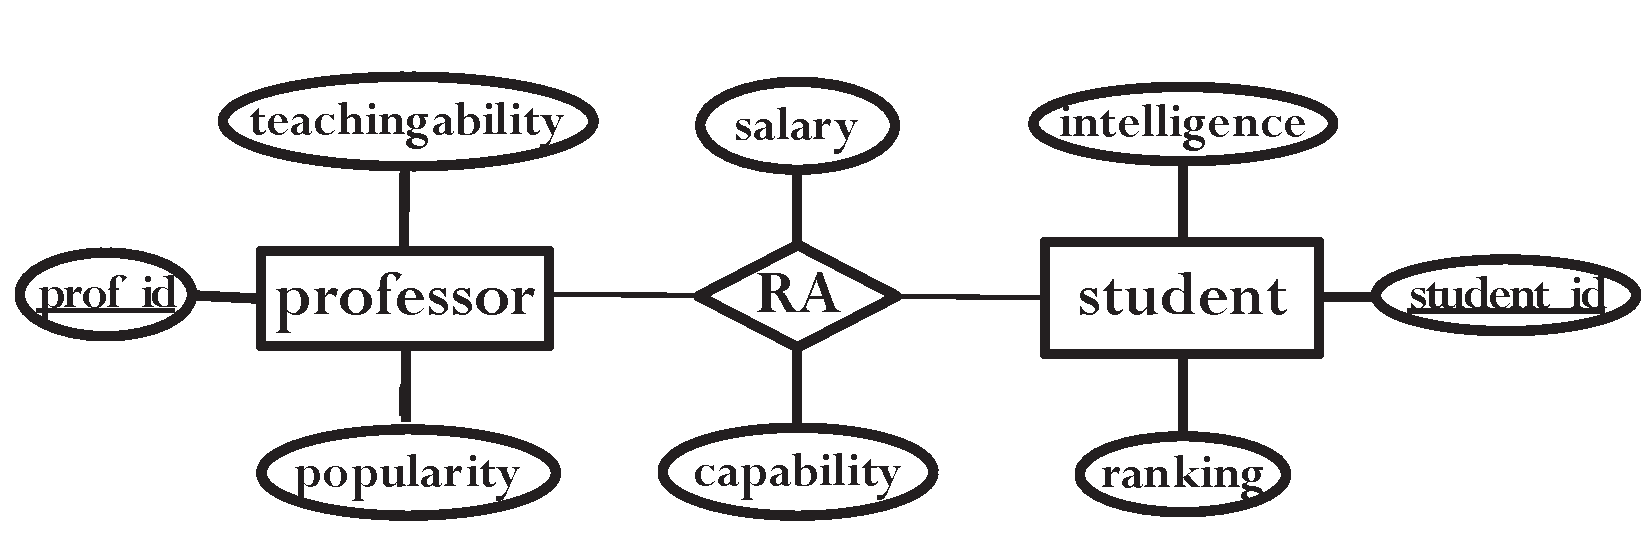
\includegraphics{university-schema.pdf} 
 } 
\caption{A relational ER Design for a university domain.}
 \label{fig:university-schema}
\end{figure}
\begin{figure}[htbp] %  figure placement: here, top, bottom, or page
 \centering
\resizebox{0.5\textwidth}{!}{
 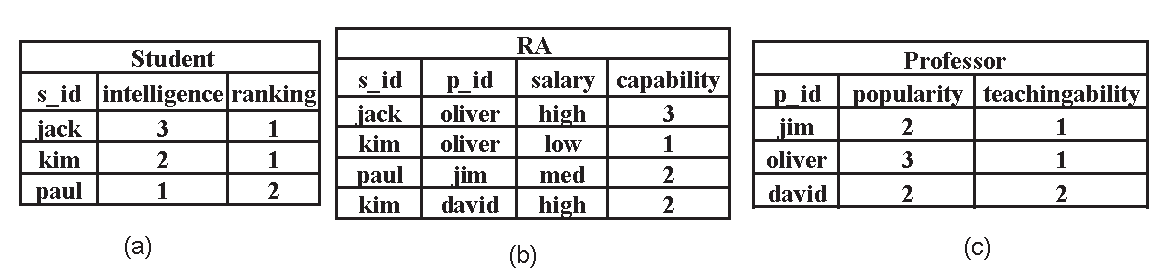
\includegraphics{university-tables.pdf} 
} 
%\caption{Database Table Instances: (a) $\student$, (b) $\course$, (c) $\prof$, (d) $\ra$, (e) $\reg$. }
\caption{Database Table Instances: (a) $\student$, (b) $\ra$, (c) $\prof$. }
 \label{fig:instance}
\end{figure}
\begin{figure}[htbp] %  figure placement: here, top, bottom, or page
 \centering
\resizebox{0.5\textwidth}{!}{
 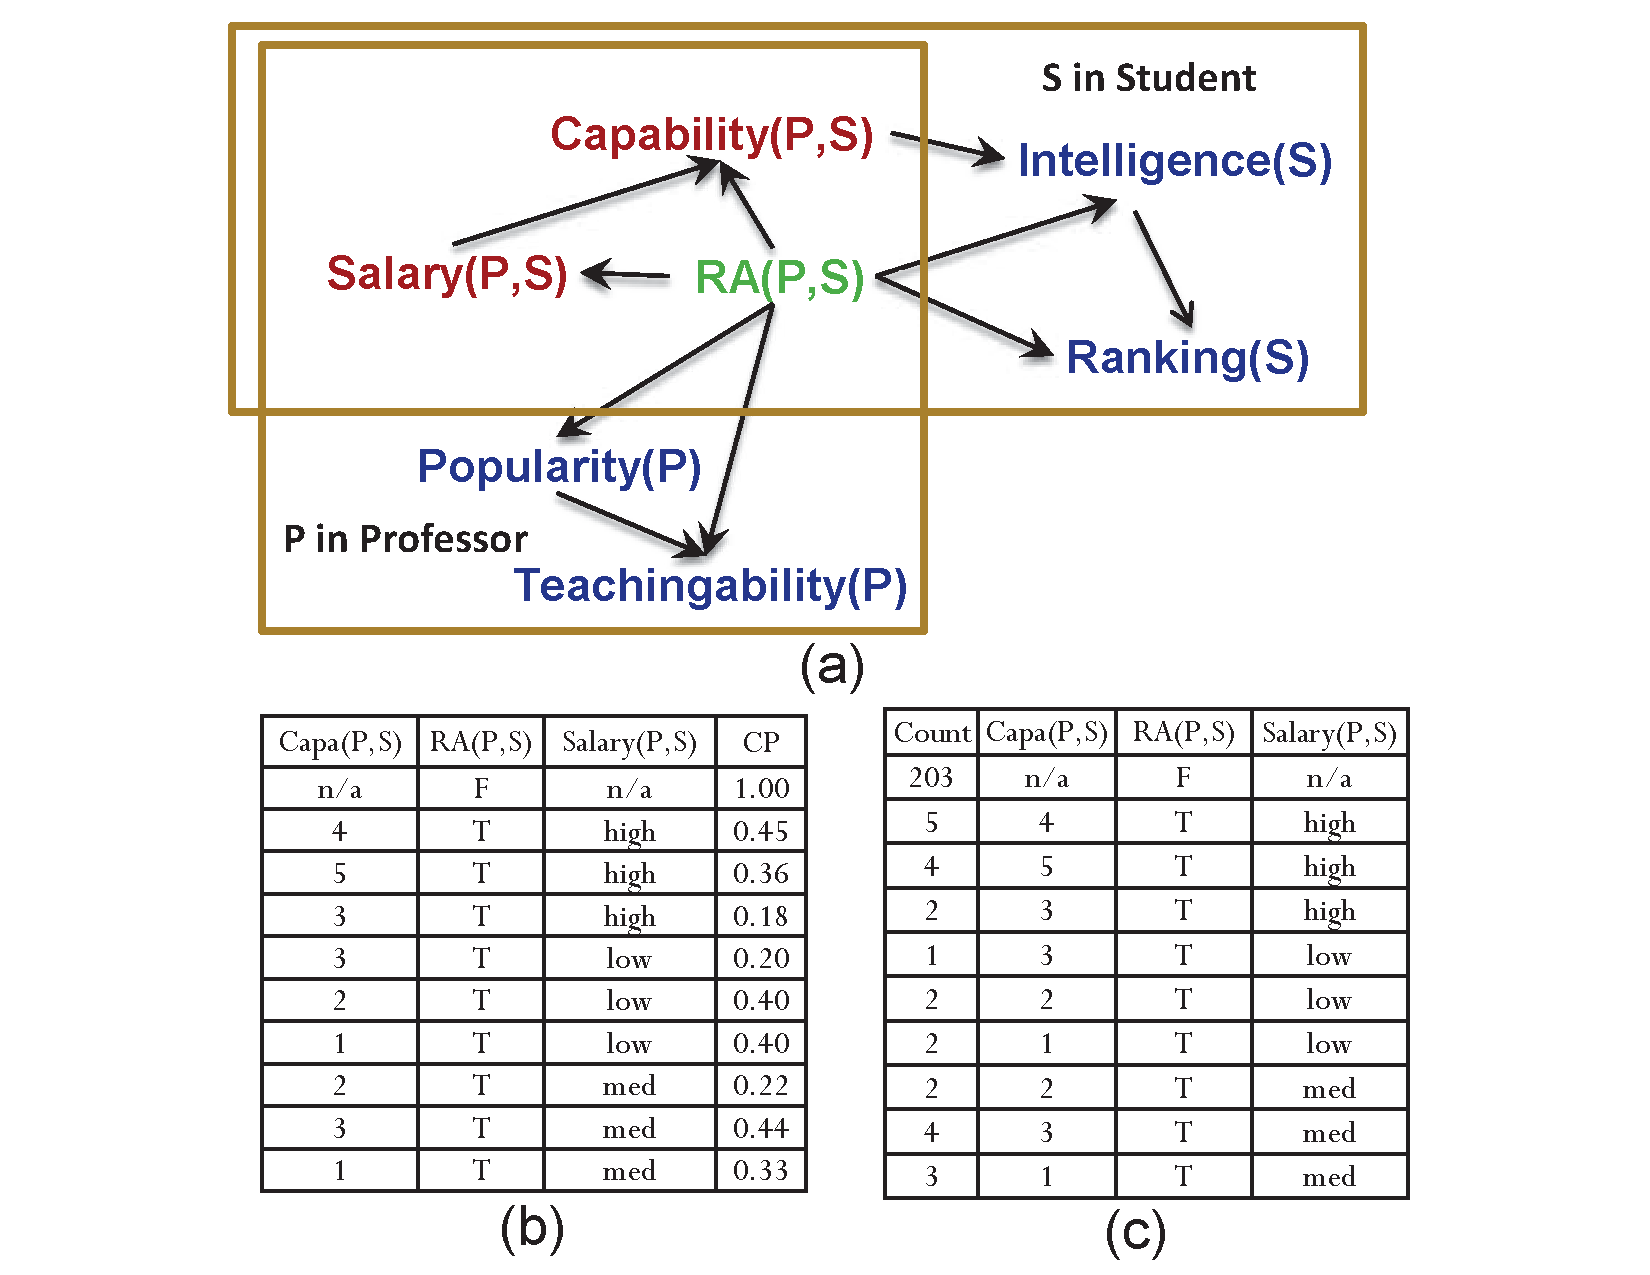
\includegraphics{pbn.pdf} 
} 
\caption{ (a) Bayesian network for the University domain. We omit the $\it{Registered}$ relationship for simplicity. The network was learned from the University dataset \cite{bib:bbsite}.
(b) Conditional Probability table $Capability(\P,\S)\_\cptable$, for the node $Capability(\P,\S)$. Only value combinations that occur in the data are shown. This is an example of a factor table. (c) Contingency Table $Capability(\P,\S)\_\cttable$ for the node $Capability(\P,\S)$ and its parents. Both CP and CT tables are stored in an RDBMS.}
% \textbf{Zhensong: must be consistent about lower-case, upper case: which one?}
 \label{fig:pbn}
\end{figure}




\section{System Overview} 

Our system design represents statistical objects as  relational tables, on a par with the original data tables, so that SQL can be used  to manage them. 
Figure~\ref{fig:architecture} represents key system components. The starting point is a multi-relational database containing the input data. 
 
\begin{figure*}[!t]
\begin{center}
\resizebox{1\textwidth}{!}{
\includegraphics
%[width=0.8\textwidth]
{pipeline}
}
\caption{System Flow. All statistical objects are stored as first-class citizens in a DBMS. Objects on the left of an arrow are utilized for constructing objects on the right. Statistical objects are constructed and managed by different modules (boxes). 
\label{fig:architecture}}
\end{center}
\end{figure*}

\subsection{The Schema Analyzer} The schema analyzer is an SQL script that queries the system catalog table to define a default set of relational random variables (par-RVs) for statistical analysis \cite{Kimmig2015}. 
%The random variables represent descriptive attributes of entities, relationships among then, and descriptive attributes of these relationships. 
The metadata include the domain of the par-RVs (possible values), and type information (possible arguments). The schema analyzer extracts metadata about the random variables from the database system catalog.
%, which includes the following information. 
%(1) The domain of the random variable. For discrete random variables, this is a finite set of possible values.
%(2) Pointers to the table and/or column in the original database that contains the data relevant to the random variables. 
The random variables and associated metadata are stored in the \textbf{random variable database} $\RVD$. We highlight two features of the $\RVD$ component. 

(i) The set of par-RVs and the associated metadata is constructed {\em automatically} from the input database. 
%In contrast, existing SRL systems require users to specify information about par-RVs and associated types, typically in a system-specific format. 
Thus \FB utilizes the data description resources of SQL to faciliate the ``setup task'' for relational learning \cite{Walker2010}.

(ii) 
%In \FB, the downstream learning algorithm and scripts query metadata only in the \RVD, not in the system catalog. 
Representing metadata explicitly offers two advantages. 
First, a user can easily edit the \RVD to customize the learning behavior, for instance by deleting irrelevant par-RVs. Second, it is possible to export metadata from other formats to the \RVD format.
%, then use \FB to perform structure learning. 
In this way \FB can serve as a structure learning backend to expressive specification languages for other relational models \cite{Guazzelli2009,Milch2005}.


%
%Statistical analysis is based on a set of random variables. Single-table data is basically self-describing with respect to random variables: each column header other than row id fields represents a random variable. In contrast, a set of data tables that represents heterogeneous multi-relational data needs to be augmented with metadata about which columns represent which entity class. Such metadata requires a {\em data description language} \cite{Ullman1982}; in SQL the relevant key concepts are primary and foreign keys. 
%%Previous work on multi-relational learning typically assumed that information about random variables for heterogeneous is specified by the user using a logical language. 
%A novel aspect of \FB is analyzing the RDBMS system catalog to translate metadata about primary and foreign keys into a specification of relational random variables. 
%
%The Schema Analyzer examines the information in the DB system catalog to define a default set of random variables for statistical analysis.  Since the system catalog is itself stored in tables, the default set of random variables can be constructed using SQL queries. Metainformation about the random variables is stored in the This database may be edited by the user to add further random variables of interest. Another possibility is for a machine learning application to create the $\RVD$ database, for example based on metainformation specified in another format.
%




\subsection{The Count Manager}

A key service for statistical-relational learning is counting how many times a given relational pattern (par-RV) is instantiated in the data. Such counts are known as {\em sufficient statistics}. 
Accessing sufficient statistics is often the main scalability bottleneck. The access patterns of a model search procedure are inherently sequential and random \cite{Niu2011}, and therefore it is important to cache sufficient statistics.  Caching is even more important if the data is stored on disk in an RDBMS, rather than in main-memory. 
%
There are several reasons for employing an RDBMS for gathering sufficient statistics. 
(1) The machine learning application saves expensive data transfer by executing count operations in the database server space rather than local main memory. (2) SQL optimizations for aggregate functions such as SUM and COUNT can be leveraged. (3) Sufficient statistics can be stored in the RDBMS. For many datasets, the number of sufficient statistics runs in the millions and is too big for main memory.  
%
%An RDBMS provides disk storage and fast access for large numbers of sufficient statistics. 
A novel aspect of \FB is managing {\em multi-relational sufficient statistics} that combine information {\em across} different tables in the relational database. This requires combining SQL aggregate functions with table joins \cite{Qian2014a}. 
 %Figure~\ref{fig:metaquery-concept} illustrates this design. 
%
%
%A novel aspect of \FB is storing sufficient statistics in contingency tables defined by database views. These views are defined by SQL queries, which are constructed using the novel concept of an SQL metaquery. An SQL metaquery takes as input the metainformation about random variables, and builds a set of tables that represent a view definition. 
\subsection{The Model Manager} 
The Model Manager supports the construction and querying of large structured statistical models, which are stored in the \textbf{Model Database} MDB. Services provided by the Model Manager include the following. (1) Compute parameter estimates for the model using the sufficient statistics in the Count Database.  (2) Computing model characteristics such as the number of parameters or degrees of freedom in a model. (3) Computing a model selection score that quantifies how well the model fits the multi-relational data. 
Model selection scores are usually functions of the number of parameters and the parameter estimates.  By employing the SQL view mechanism, parameter estimates and model selection scores are updated automatically during the model search.
\section{Conclusion}
Compared to traditional learning with a single data table, learning for multi-relational data requires new system capabilities. In this paper we described \FB, a system that leverages the existing capabilities of an SQL-based RDBMS to support statistical-relational learning.
Representational tasks include specifying metadata about structured first-order random variables, and storing the structure of a learned model. Computational tasks include storing and constructing sufficient statistics, and computing parameter estimates and model selection scores. 
We showed that SQL scripts can be used to implement these capabilities, with multiple advantages. These advantages include: 1) Fast program development through high-level SQL constructs for complex table and count operations. 2) Managing large and complex statistical objects that are too big to fit in main memory. 
For instance, some of our benchmark databases require storing and querying millions of sufficient statistics. While \FB\ provides good solutions for each of these system capabilities in isolation, the ease with which large complex statistical-relational objects can be integrated via SQL queries is a key feature. 

{\em Future Work.} Further potential application areas for \FB\ include managing massive numbers of aggregate features for classification \cite{Popescul2007}, and collective matrix factorization \cite{Singh2008}. An important goal is a single RDBMS package for both learning and inference that integrates \FB\ with inference systems such as BayesStore and Tuffy. 

There are opportunities for optimizing RDBMS operations for the workloads required by statistical-relational structure learning. These include view materialization and the key scalability bottleneck of computing multi-relational sufficient statistics. There are several fundamental system design choices whose trade-offs for SRL warrant exploration. These include the choice between pre-counting and post-counting sufficient statistics, and using main memory vs. RDBMS disk storage. For instance, model selection scores can be cached in either main memory or the database. Our SQL-based approach facilitates using distributed computing systems such as SparkSQL \cite{Michael2015}, which have shown great potential for scalability. 

%\section{Examples} \label{sec:examples} SRL has developed a number of formalisms for describing par-factors \cite{Kimmig2015}. 
%One option is to use SQL queries, as in Relational Markov networks \cite[Sec.3.2.1]{Kimmig2015}, another to use first-order logic (FOL) formulas, as in Markov Logic Networks \cite{Domingos2009}. 
%The model structure is a set of FOL formulas, and the parameters specify a weight for each. A grounding of an FOL formula with weight $w$ represents a value assignment to a ground set of par-RVs, with associated factor value $e^{w}$. 
%First-order probabilistic graphical models
%are popular both within SRL and the database community \cite{Kimmig2015,Wang2008}. The model structure is defined by edges connecting par-RVs. For instance, a \textbf{parametrized Bayesian network structure} is a directed acyclic graph whose nodes are par-RVs.  Figure \ref{fig:pbn} shows a Bayesian network for a University domain. We use the university example as a toy running example throughout the paper. The schema for the university domain is given in Figure~\ref{fig:university-schema}. This schema features only one relationship for simplicity; \FB\ learns a model for any number of relationships. While we describe \FB\ abstractly in terms of par-factors, for concreteness we illustrate it using Bayesian networks. The system takes as input a database instance like that shown in Figure~\ref{fig:instance}, and produces as output a graphical model like that shown in Figure~\ref{fig:pbn}.  


%For this instance, there are three possible ground random variables of the par-RV $\it{Popularity}(\P)$, namely $\it{Popularity}(\it{jim}), \it{Popularity}(\it{oliver}), \it{Popularity}(\it{david})$. 
%A par-factor in a Bayesian network is associated with a \textbf{family} of nodes \cite[Sec.2.2.1]{Kimmig2015}. A family of nodes comprises a child node and all of its parents. For example, in the BN of Figure~\ref{fig:pbn}, one of the par-factors is associated with the par-RV set $\parrvs=\{\it{Capability}(\P,\S),\it{Salary}(\P,\S),\it{RA}(\P,\S)\}$. For the database instance of Figure~\ref{fig:instance}, there are $3\times3=9$ possible factors associated with this par-RV, corresponding to the Cartesian product of 3 professors and 3 students. The value of the factor $\phi$ is a function from an assignment of family node values to a non-negative real number. {\em In a Bayesian network, the factor value represents the conditional probability of the child node value given its parent node values.} These conditional probabilities are typically stored in a table as shown in Figure~\ref{fig:pbn}(b). This table represents therefore the function $\phi$ associated with the family par-factor. Assuming that all par-RVs have finite domains, a factor can always be represented by a \textbf{factor table} of the form Figure~\ref{fig:pbn}(b): there is a column for each par-RV in the factor, each row specifies a joint assignment of values to a par-RV, and the factor column gives the value of the factor for that assignment (cf. \cite[Sec.2.2.1]{Kimmig2015}).


%To evaluate a joint probability $P(\set{X}=\set{x})$ over all ground par-RVs using Equation~\ref{eq:parfactor}, we must count the number of times that each row in the CP-table is instantiated in the joint assignment $\set{X}=\set{x}$. 
%The sufficient statistics for the $\it{Capability}(\P,\S)$ family can be represented in a contingency table as shown in Figure~\ref{fig:pbn}(c). For example, the first row of the contingency table indicates that the conjunction $\it{Capability}(\P,\S)=n/a,\it{Salary}(\P,\S)=n/a,\it{RA}(\P,\S) =\false$ is instantiated 203 times in the University database (publicly available at~\cite{bib:bbsite}). This means that for 203 professor-student pairs, the professor did not employ the student as an RA (and therefore the salary and capability of this RA relationship is undefined or $n/a$).
%
%\subsection{SRL Structure Learning}
%
%Algorithm~\ref{alg:learning} shows the generic format of a statistical-relational structure learning algorithm (adapted from 
%\cite{Kimmig2015}%Kimming and Getoor
%). The instantiation of procedures in lines 2, 3, 5 and 8 determines the exact behavior of a specific learning algorithm. The structure algorithm carries out a local search in the hypothesis space of graphical relational models. A set of candidates is generated based on the current model (line 3), typically using a search heuristic. For each candidate model, parameter values are estimated that maximize a model selection score function chosen by the  user (line 5). A model selection score is computed for each model given the parameter values, and the best-scoring candidate model is selected (line 7). 
%We next discuss our system design and how it supports model discovery algorithms that follow the outline of Algorithm~\ref{alg:learning}. Figure~\ref{fig:architecture} outlines the system components and dependencies among them.

%\begin{algorithm}[htbp]
%%\label{Pivot_CT_Computation}
%
%\KwIn{Hypothesis space $ \mathcal H$ (describing graphical models), training data $\mathcal D$ (assignments to random variables), scoring function score ($\cdot$, $\mathcal D$)}
%\KwOut{A graph structure $G$ representing par-factors.}
%\begin{algorithmic}[1]
%\STATE $\mathcal G \leftarrow 	\emptyset$
%%$ $ h \leftarrow 	\emptyset ;$
%\WHILE{ \textsc{continue}($\mathcal G$, %$h$, 
%$\mathcal H$, score ($\cdot$, $\mathcal D$) )} 
%	\STATE{ $\mathcal R \leftarrow $ \textsc{refine}C\textsc{andidates}($\mathcal G, \mathcal H$)} 
% 	\FORALL{$R \in \mathcal R$} 
%		\STATE{$R \leftarrow$ \textsc{learn}P\textsc{arameters}($R$,score ($\cdot$, $\mathcal D$))} 
%    \ENDFOR
%	\STATE 	$\mathcal G \leftarrow$ argmax$_{G^{\prime} \in \mathcal R\cup \{G\}}$ score($G^{\prime} $, $\mathcal D$)
%%
%%	$h \leftarrow$ arg max$_{h^{\prime} \in \mathcal R\cup \{h\}}$ score($h^{\prime} $, $\mathcal D$)
%%	\STATE $\mathcal G \leftarrow \textsc{select}$($ \mathcal R$, score ($\cdot$, $\mathcal D$))
%\ENDWHILE
%
%%\COMMENT{Implements the algebra Equation~\ref{update} in proposition~\ref{PivotCT}.}
%\STATE \Return $G$
%\end{algorithmic}
%\label{alg:learning}
%\caption{Structure learning algorithm 
%%(instantiation of procedures in lines 2, 3, 5 and 8 determines exact behavior) 
%}
%\end{algorithm}
%

%\begin{algorithm}[htbp]
%%\label{Pivot_CT_Computation}
%
%\KwIn{Hypothesis space $ \mathcal H$ (describing graphical models), training data $\mathcal D$ (assignments to random variables), scoring function score ($\cdot$, $\mathcal D$)}
%\KwOut{A graph structure $G$ representing par-factors.}
%\begin{algorithmic}[1]
%\STATE $G \leftarrow 	\emptyset$
%%$ $ h \leftarrow 	\emptyset ;$
%\WHILE{ \textsc{continue}($G$, %$h$, 
%$\mathcal H$, score ($\cdot$, $\mathcal D$) )} 
%	\STATE{ $\mathcal R \leftarrow $ \textsc{refine}C\textsc{andidates}($G, \mathcal H$)} 
% 	\FORALL{$R \in \mathcal R$} 
%		\STATE{$R \leftarrow$ \textsc{learn}P\textsc{arameters}($R$,score ($\cdot$, $\mathcal D$))} 
%    \ENDFOR
%	\STATE 	$G \leftarrow$ argmax$_{G^{\prime} \in \mathcal R\cup \{G\}}$ score($G^{\prime} $, $\mathcal D$)
%%
%%	$h \leftarrow$ arg max$_{h^{\prime} \in \mathcal R\cup \{h\}}$ score($h^{\prime} $, $\mathcal D$)
%%	\STATE $G \leftarrow \textsc{select}$($ \mathcal R$, score ($\cdot$, $\mathcal D$))
%\ENDWHILE
%
%%\COMMENT{Implements the algebra Equation~\ref{update} in proposition~\ref{PivotCT}.}
%\STATE \Return $G$
%\end{algorithmic}
%\label{alg:learning}
%\caption{Structure learning algorithm 
%%(instantiation of procedures in lines 2, 3, 5 and 8 determines exact behavior) 
%}
%\end{algorithm}
\bibliographystyle{unsrt}
\bibliography{master} 

\end{document}
%\subsubsection*{Acknowledgments}
%
%Use unnumbered third level headings for the acknowledgments. All
%acknowledgments go at the end of the paper. Do not include 
%acknowledgments in the anonymized submission, only in the 
%final paper. 
%
%\subsubsection*{References}
%
%References follow the acknowledgments. Use unnumbered third level heading for
%the references. Any choice of citation style is acceptable as long as you are
%consistent. It is permissible to reduce the font size to `small' (9-point) 
%when listing the references. {\bf Remember that this year you can use
%a ninth page as long as it contains \emph{only} cited references.}
%
%\small{
%[1] Alexander, J.A. \& Mozer, M.C. (1995) Template-based algorithms
%for connectionist rule extraction. In G. Tesauro, D. S. Touretzky
%and T.K. Leen (eds.), {\it Advances in Neural Information Processing
%Systems 7}, pp. 609-616. Cambridge, MA: MIT Press.
%
%[2] Bower, J.M. \& Beeman, D. (1995) {\it The Book of GENESIS: Exploring
%Realistic Neural Models with the GEneral NEural SImulation System.}
%New York: TELOS/Springer-Verlag.
%
%[3] Hasselmo, M.E., Schnell, E. \& Barkai, E. (1995) Dynamics of learning
%and recall at excitatory recurrent synapses and cholinergic modulation
%in rat hippocampal region CA3. {\it Journal of Neuroscience}
%{\bf 15}(7):5249-5262.
%}

\end{document}
